\documentclass{article}
\usepackage{amsmath,amsthm,amssymb}
\usepackage{mathtext}
\usepackage[T2A]{fontenc}
\usepackage[utf8]{inputenc}
\usepackage[english]{babel}
\usepackage{graphicx}
\usepackage{hyperref}


\title{Russian address elements classification using artificial neural networks}
\author{Anton Reshetnikov}
\date{May 2024}



\begin{document}
\maketitle
\begin{abstract}
    This documents provides result of research of token classification task applied to russian place addresses.
    The task is to recognize elements of address like region, area, city, territory, street.
    The source code available at
     \url{https://github.com/qwazer/ruaddress-elements-classification}.
\end{abstract}



\section{Introduction}


Logistics companies have the task of checking and normalizing the address against the incoming string.
For example, there is an input string with the address ``Москва, Абрат, 1'' (in Russian).
It is necessary to select address-forming elements, check against the database,
that such an address actually exists and return the status of the address and its normalized representation.

Traditionally, IT systems that solve this problem using a rules-based approach (word level tokenization, token classification by regular expressions).
The task is to explore the possibilities of solving the same problem using modern deep learning models.

\subsection{Team}

\textbf{Anton Reshetnikov} - researcher



\section{Related Work}
\label{sec:related}
\cite{makarov2020algo} provides overview of traditional algorithms used for address elements recognition.
The particular solution for address element recognition described in ~\cite{habr2020gar}
%todo overview of international attempts

\section{Model Description}

The most modern deep learning models based on Transformer architecture described in the ``Attention Is All You Need'' article~\cite{vaswani2023attention}.
There are several models adapted for russian language exists.
For detail see this overview article:~\cite{zmitrovich2024family}.

For the purpose of current research \href{https://huggingface.co/cointegrated/rubert-tiny2}{cointegrated/rubert-tiny2} model selected.
Reasons of such choice are:
\begin{enumerate}
    \item It based on Transformer architecture;
    \item The model is focused on Russian;
    \item Small size, which make it suitable for fast experiments.
\end{enumerate}


\section{Dataset}

\subsection{Datasource}
The dataset based on freely available ``State address register'' distributed at \url{https://fias.nalog.ru/} by Federal Taxation Service of the Russian Federation.

Only address elements related to Administrative division (Административно-территориальное деление) was selected from the ``State address register''.

\subsection{Token classes}

Dictionary ``Element type'' used as token classes for token classification task.
Values of dictionary are:
\begin{enumerate}
    \item REGION
    \item REGION\_TYPE
    \item AREA
    \item AREA\_TYPE
    \item TERRITORY
    \item TERRITORY\_TYPE
    \item CITY
    \item CITY\_TYPE
    \item STREET
    \item STREET\_TYPE
    \item DELIMITER
\end{enumerate}

\subsection{Mapping table}
Address elements levels of ``State address register'' mapped to custom dictionary ``Element type'' with next mapping table:


\begin{center}
    \begin{tabular}{| l | l | l | }
        \hline
        State address register level (in Russian) & Element type & Example  \\
        \hline
        Субъект & REGION & Омская область  \\
        Административный район & AREA & Любинский р-н   \\
        Город & CITY &    \\
        Населенный пункт & CITY &  поселок Камышловский \\
        Элемент планировочной структуры & TERRITORY & Территория СНТ Сибзаводовец-2  \\
        Элемент улично-дорожной сети & STREET & 7-я аллея \\
        Земельный участок & not used & \\
        Здание (сооружение) & not used &  \\
        Помещение & not used & \\
        Помещения в пределах помещения & not used  &\\
        Машино-место & not used  &\\
        \hline
    \end{tabular}
\end{center}

In case of REGION and CITY has the same value (like for ``город Москва'', ``город Санкт-Петербург'', ``город Севастополь'', ``город Байконур'') CITY tokens are omitted.

\subsection{Dataset structure}

The idea is to generate own dataset called ``Ruaddress'' from ``State address register'' datasource.
The ``Ruaddress'' dataset has 2 columns, described in the next table:

\begin{center}
    \begin{tabular}{| l | p{6cm} | l | }
        \hline
        Column name & tokens & classes  \\
        Description & list of token words & list of class codes  \\
        Example & [Вологодская, Область,,, Грязовецкий, Район, Вохтога, Рабочий, поселок] &  [1, 2, 11, 3, 4, 7, 8, 8] \\
        \hline
    \end{tabular}
\end{center}



\subsection{Augmenation}

A place address can be presented in a various forms.
To generate address form from address elements the augmentation procedure is used.
The procedure receive address-forming elements for a place, then apply series of transformation and output 2 lists: tokens and related token classes.

\subsubsection{Formats of address element}

Controlled by next options:

\begin{center}
    \begin{tabular}{| l | l | l |  l | }
        \hline
        Option & Probability & Example for True value & Example for False value \\
        \hline
        typeFirst & 0.75 & поселок Мирный & Завьяловский район  \\
        commaSeparator & 0.75 & поселок Мирный\textbf{,} & Завьяловский район  \\
        shortType & 0.5 & п. Мирный\textbf{,} & Завьяловский р-н  \\
        \hline
    \end{tabular}
\end{center}



\subsubsection{Char level augmentation}

For adding some noise and corruptions to the words the \href{https://github.com/ai-forever/augmentex}{augmentex} tool used.
The augmentex tool described in next paper \cite{martynov2023augmentation}.
It used with next config:

\begin{verbatim}
char_aug = CharAug(
    unit_prob=0.05, # Percentage of the phrase to which augmentations will be applied
    min_aug=0, # Minimum number of augmentations
    max_aug=3, # Maximum number of augmentations
    mult_num=3, # Maximum number of repetitions of characters
    random_seed=42,
    lang="rus", # supports: "rus", "eng"
    platform="pc", # supports: "pc", "mobile"
)

\end{verbatim}

\subsubsection{Word shortening}

For word shortening 2 options are used.


\begin{center}
    \begin{tabular}{| l | l | l |  l | }
        \hline
        Option & Probability & Example for Красноярский & \\
        \hline
        hyphen substition & 0.15 & Красн-кий  \\
        dot truncation & 0.15 & Красн.  \\
        \hline
    \end{tabular}
\end{center}


\subsection{``Ruaddress'' dataset}

The ``Ruaddress'' dataset consist of 1,5 millions augmented addresses.
The dataset was split on train, test, validation parts in 4:1:1 (0.66:0.16:0.16) proportion accordingly.


\section{Experiments}

The model was trained using Jupiter notebook  from the ~\cite{nlpcourse2022} article.
The original Jupiter notebook from Hugging face NPL course was adapted for the ``Ruaddress'' dataset.



\subsection{Metrics}
Standard metrics for classification task are used: Precision, Recall, F1.

\subsection{Experiment Setup}

The experiments shown that the model can be effectively trained in 1 epoch.
The second epoch and the third epoch increase metrics in less than 0,005 \%.

The whole list of parameters are shown in the next code snippet

\begin{verbatim}
args = TrainingArguments(
    "bert-finetuned-ner",
    evaluation_strategy="epoch",
    save_strategy="epoch",
    learning_rate=2e-5,
    num_train_epochs=1,
    weight_decay=0.01
)
\end{verbatim}


\section{Results}

The trained model solve address token classification task.

Example

Input:
\begin{verbatim}
Ставропольский край г Лермонтов территория
садоводческого некоммерческого товарищества
имени И.В. Мичурина, ул массив 3 линия 3
\end{verbatim}
Output:
\begin{verbatim}
    REGION - Ставропольский
    REGION_TYPE - край
    CITY_TYPE - г
    CITY - Лермонтов
    TERRITORY_TYPE - территория
    TERRITORY - садоводческого некоммерческого товарищества имени И. В. Мичурина
    DELIMITER - ,
    STREET_TYPE - ул
    STREET - массив 3 линия 3
\end{verbatim}

The model published to huggingface at \href{https://huggingface.co/qwazer/rubert-address-elements}{qwazer/rubert-address-elements}.
The example of Inference API output show on Fig.~\ref{fig:inference-example}

\begin{figure}[!tbh]
    \centering
    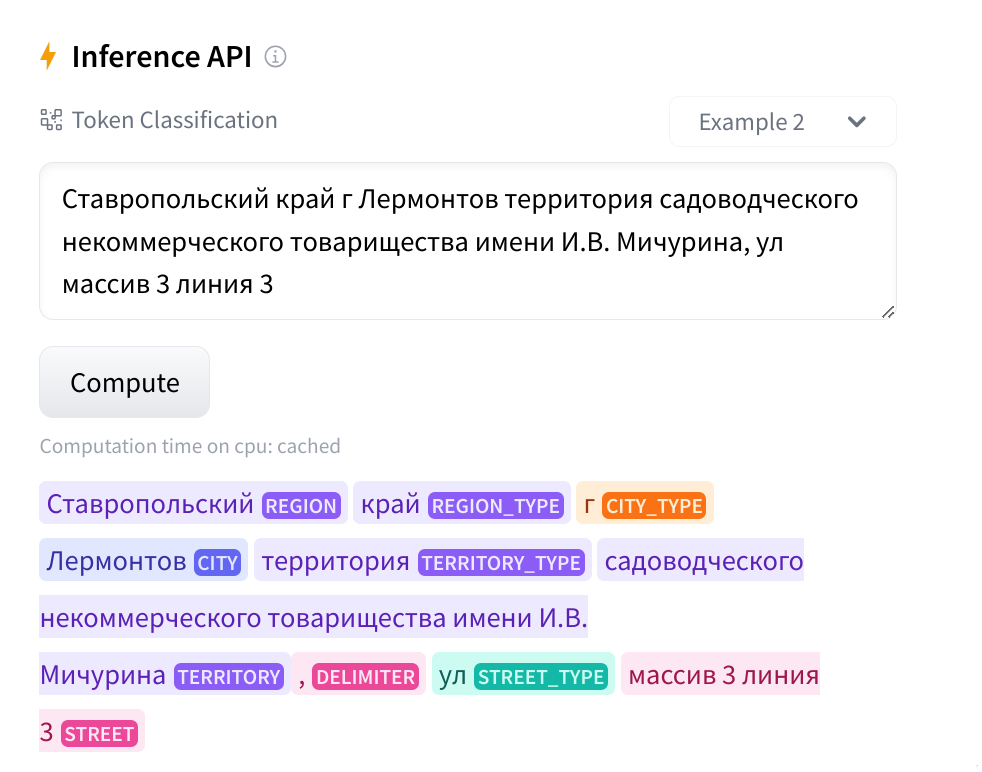
\includegraphics[width=1\linewidth]{inference-example-02}
    \caption{Inference example}
    \label{fig:inference-example}
\end{figure}

The comparisons with other models was not performed in scope of the current work.


\section{Conclusion}

In scope of the current work the ``Ruaddress'' dataset based on ``State address register'' was build.
It was augmented using different techniques.
The model \href{https://huggingface.co/cointegrated/rubert-tiny2}{cointegrated/rubert-tiny2}
was fine-tined for the token classification task applied to russian place addresses.
The resulting model was published to huggingface at \href{https://huggingface.co/qwazer/rubert-address-elements}{qwazer/rubert-address-elements}.

\subsection{Futher steps and ideas to improve the model}
\begin{enumerate}
    \item Add more tokens for buildings, steads, flats, possible inclusion of person or organization names, etc.
    \item More word-level augmentations like word drop, swap, etc
    \item Support for translit
    \item Build the model bases on Recurrent networks and compare metrics and performance.
    \item Try to build multi-classification model, when a word can have multiple tokens.
\end{enumerate}



\bibliographystyle{apalike}
\bibliography{lit}
\end{document}